%!TEX root = ../thesis.tex
\subsection{Results of Formative Study}

\begin{figure*}[t]
  \centering
  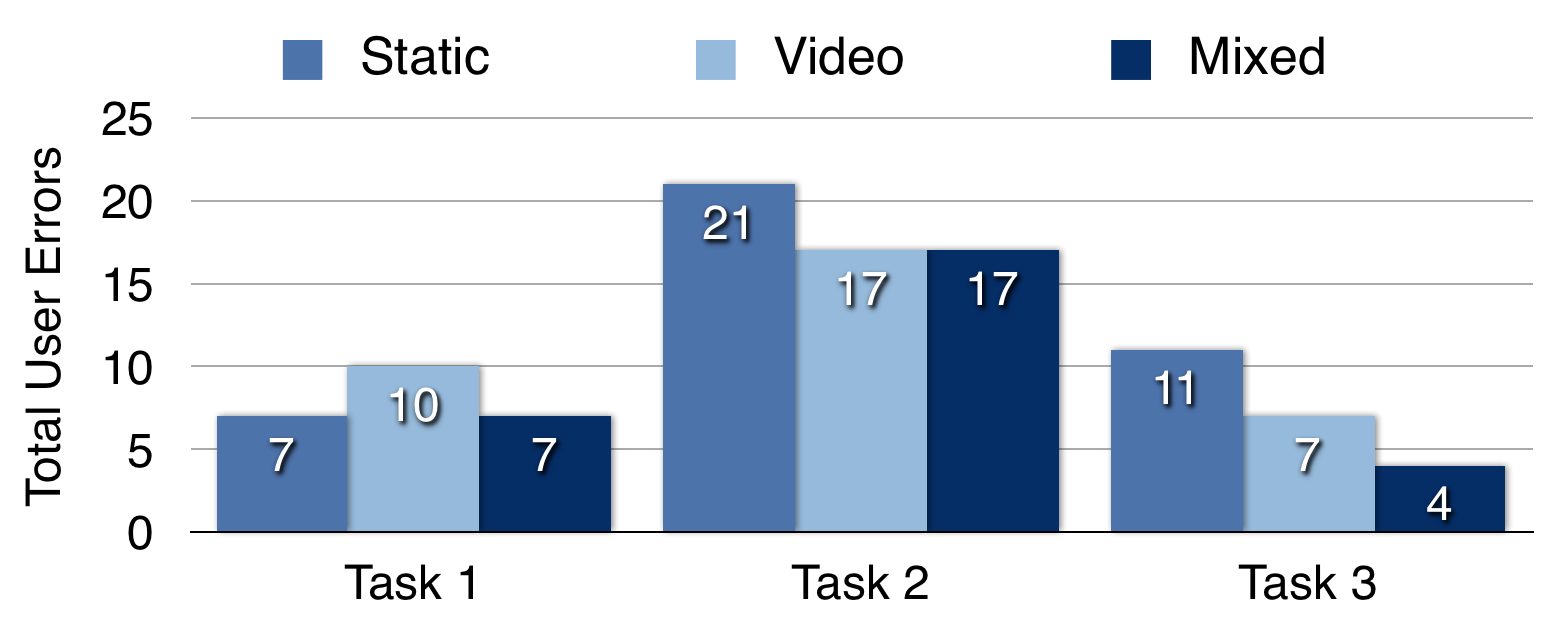
\includegraphics[width=0.5\textwidth]{\mixt/fig/formative_study/study-errors3}
  \caption{Users tied for fewer errors with mixed tutorials.}
  \label{fig:formative_errors}
\end{figure*}

\begin{figure*}[t]
  \centering
  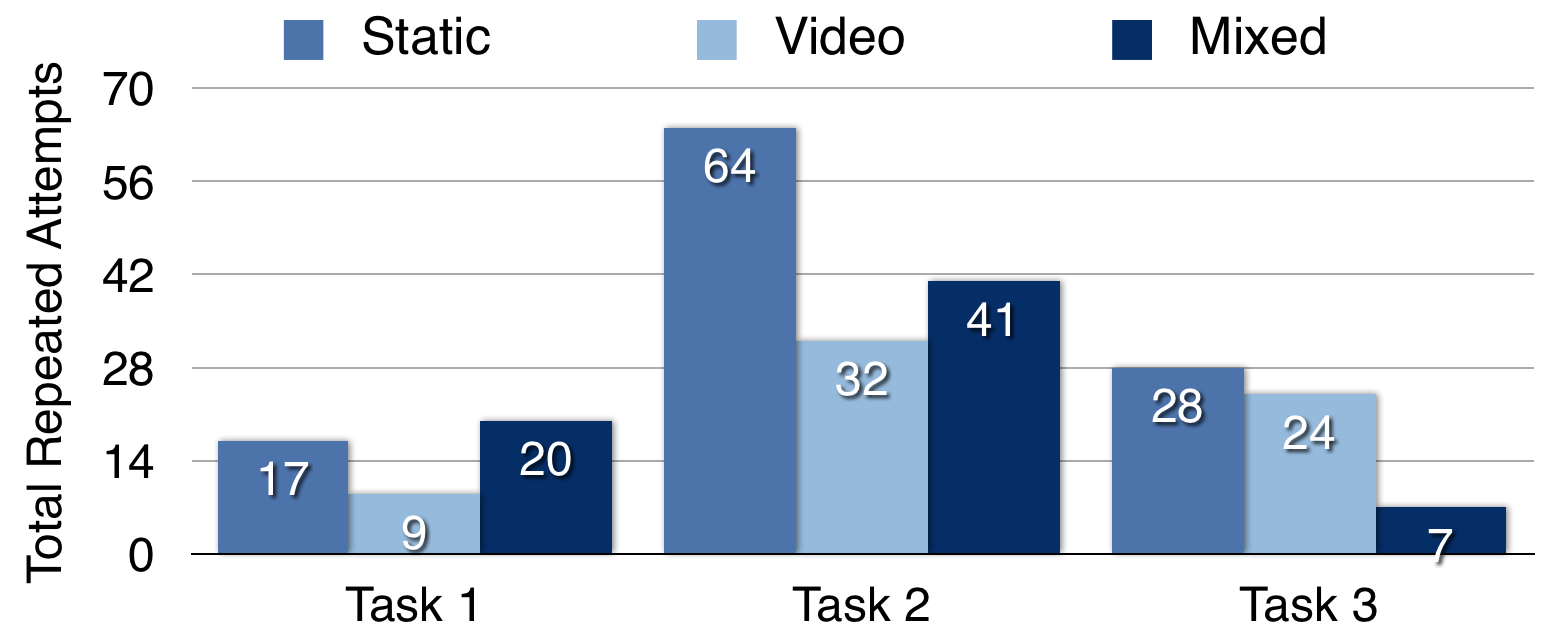
\includegraphics[width=0.5\textwidth]{\mixt/fig/formative_study/study-repeats3}
  \caption{In two of three tasks, participants made more repeated attempts at executing steps with static tutorials than with mixed tutorials. Video tutorials had the fewest attempts.}
  \label{fig:formative_attempts}
\end{figure*}

Based on the quantitative data and observations from our study, we gained several insights about how users interact with static and video content.

\subsubsection{User Performance on Image Editing Tasks}
Our analysis of user performance supports \textbf{H1}. As Figure~\ref{fig:formative_errors} shows, mixed tutorials resulted in the fewest total number of errors (28 for mixed, 34 for video, 39 for static) across all three tasks and produced an equivalent or fewer number of errors compared to static and video for any given task. In terms of extraneous work, the mixed condition resulted in many fewer repeated attempts than static tutorials and slightly more than video tutorials (65 for video, 68 for mixed, 109 for static, see Figure~\ref{fig:formative_attempts}). Although the differences in errors and repeated attempts are not statistically significant–-likely due to the small study size and differences between the tasks-–the overall trends suggest that mixed tutorials help users make fewer errors and do less extraneous work compared to static and video tutorials.

In addition to these quantitative results, we observed a few specific behaviors that had an impact on user performance:

The scannable nature of the static and mixed tutorial formats helped users follow along and avoid missing steps that might result in errors. In the video condition, users were more likely to accidentally skip steps because they were working at a different pace than the video. They also had trouble finding previous steps when trying to identify the source of an error.

In the static condition, users had trouble understanding how to perform steps that involve complex or unfamiliar UI elements and interactions. As we discuss in the following subsection, these were often the same steps where users decided to play the videos in the mixed condition. With only static text and images, users often made errors or had to repeat such steps multiple times.

Participants used the video clips in the mixed condition in a few different ways. Some users played the video \emph{before} attempting the step to familiarize themselves with the relevant UI elements and interactions. In some cases, users also played the video at the same time as they performed the action, which corresponds to what Palmiter and Elkerton described as ``mimicking actions'' \cite{Palmiter:1991:ADV:107792.107797}. We suspect both of these behaviors helped reduce errors, especially for complex or unfamiliar steps. In addition, several users also played the video \emph{after} completing a step, as a way to confirm that they had performed the step correctly and “debug” what went wrong if they made an error. This confirmation behavior helped reduce repeated attempts by making it easier to recognize and fix errors sooner.

In some cases, users had trouble seeing all of the relevant details in the mixed videos because the videos were scaled down to 800x500 pixels. For example, when using the \emph{puppet warp} tool, users missed that dragging in the vicinity of a control point (instead of on top of the control point) initiated a control wheel for a rotation rather than a translation maneuver. Although participants neither complained about not being able to resize the video in the MixT condition nor chose full-screen mode in the video condition, they explained that they would hope to clearly see the key part of the demonstration video.

\begin{table}[t]
  \centering
  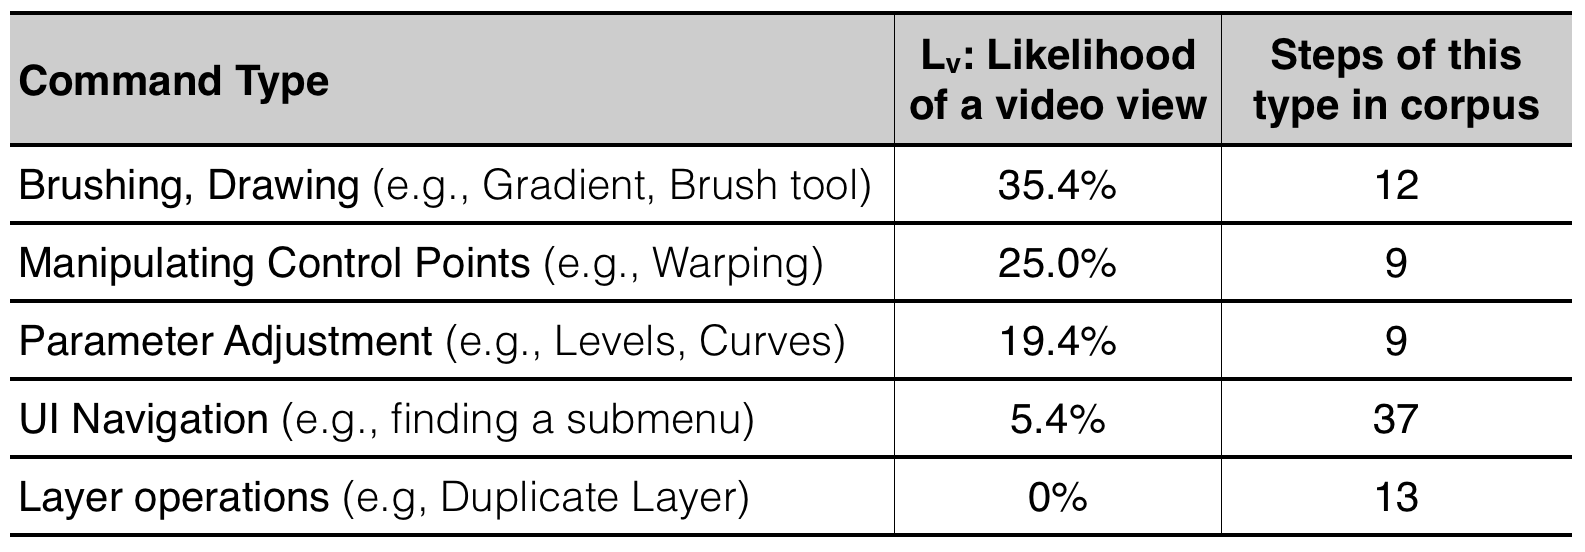
\includegraphics[width=0.8\columnwidth]{\mixt/fig/formative_study/command-table2}
  \caption{Participants watched videos most often for brushing, control point manipulation, and parameter adjustments.}
  \label{tab:formative_video_views}
\end{table}

\subsubsection{Which Commands Led to Video Views?}
Our analysis of which mixed steps prompted users to click on the corresponding videos suggests that users did indeed find the video clips more beneficial for some types of steps over others (\textbf{H2}). To compute the \emph{likelihood of a video view} ($L_V$) for the five command categories described earlier, we first determine $L_V$ for each individual step (across all three mixed tutorials) by computing the fraction of users who clicked to view the video for that step, and then we average likelihoods across all the steps in each command category.

As Table~\ref{tab:formative_video_views} shows, $L_V$ is highest for steps that involve brushing/drawing, manipulating control points and parameter adjustments. Based on our observations, videos help users perform the first two types of commands (brushing/drawing and manipulating control points) by explicitly demonstrating the necessary mouse movements rather than requiring the user to infer what to do from text and images alone. In addition, we noticed that some participants used the video clips to determine how precise they needed to be for certain brushing or selection tasks, which is hard to convey with a static representation. Text descriptions such as ``rough'' and ``detailed'' are relative and can be interpreted differently by individuals, but seeing how much time the demonstrator devotes to the task provides a much clearer estimate of the required precision for that task. As for parameter adjustments, users may be relying on the videos to provide some context about the range of visual effects the relevant parameters cover in order to determine what parameter values to use for their own image. Unlike static images, which only show the final parameter values and resulting effect, video demonstrations often show how the canvas changes as continuous parameters are updated (often via sliders), which may give users a better sense for the desired outcome of the step.

\subsubsection{User Preferences for Tutorial Types}
The results of our questionnaire show that while participants had varying opinions on the static and video tutorials, all users strongly agreed that the mixed tutorial was easy to follow. Participants had difficulty finding the tools that the static tutorials referenced and remarked that there were not enough visuals. For full-length videos, participants disliked having to pause the video to complete each step. For the mixed tutorial, half the participants found that video was the most useful among different media components for understanding a step instruction. One participant acknowledged that because the mixed tutorial allowed him to “break down the process into simple steps,” he was able to easily find the point where he had made a mistake. Another user explained that videos would be most helpful if the tasks were more advanced and in-depth. On the other hand, users had different preferences within a task. Expertise could be tool-specific: users might find static instructions sufficient for one set of operations (e.g., duplicating layers), and needed to watch videos for another set they were less familiar with (e.g., the \emph{puppet warp} tool). Overall, these responses suggest that users appreciated being able to choose from static and video features in mixed tutorials.


